\chapter{Order-of-convergence validation}
\label{chap:validation}

\section{One-dimensional convergence study}

The principal order study uses \(n=50,100,200,400,800,1600\) and two smooth
periodic advection profiles. This setting isolates reconstruction and time
integration before multidimensional flux divergence is introduced. The
method-dependent CFL policy is the same as in the later experiments:
\(\mathrm{CFL}=0.40\) for WENO-2 and WENO-3 and \(\mathrm{CFL}=0.25\) for
ADER-3. Figure~\ref{fig:conv1d} gives the overall error trend, while
Tables~\ref{tab:conv1d-smooth} and~\ref{tab:conv1d-gaussian} retain every
measured local order.

\begin{figure}[H]
\centering
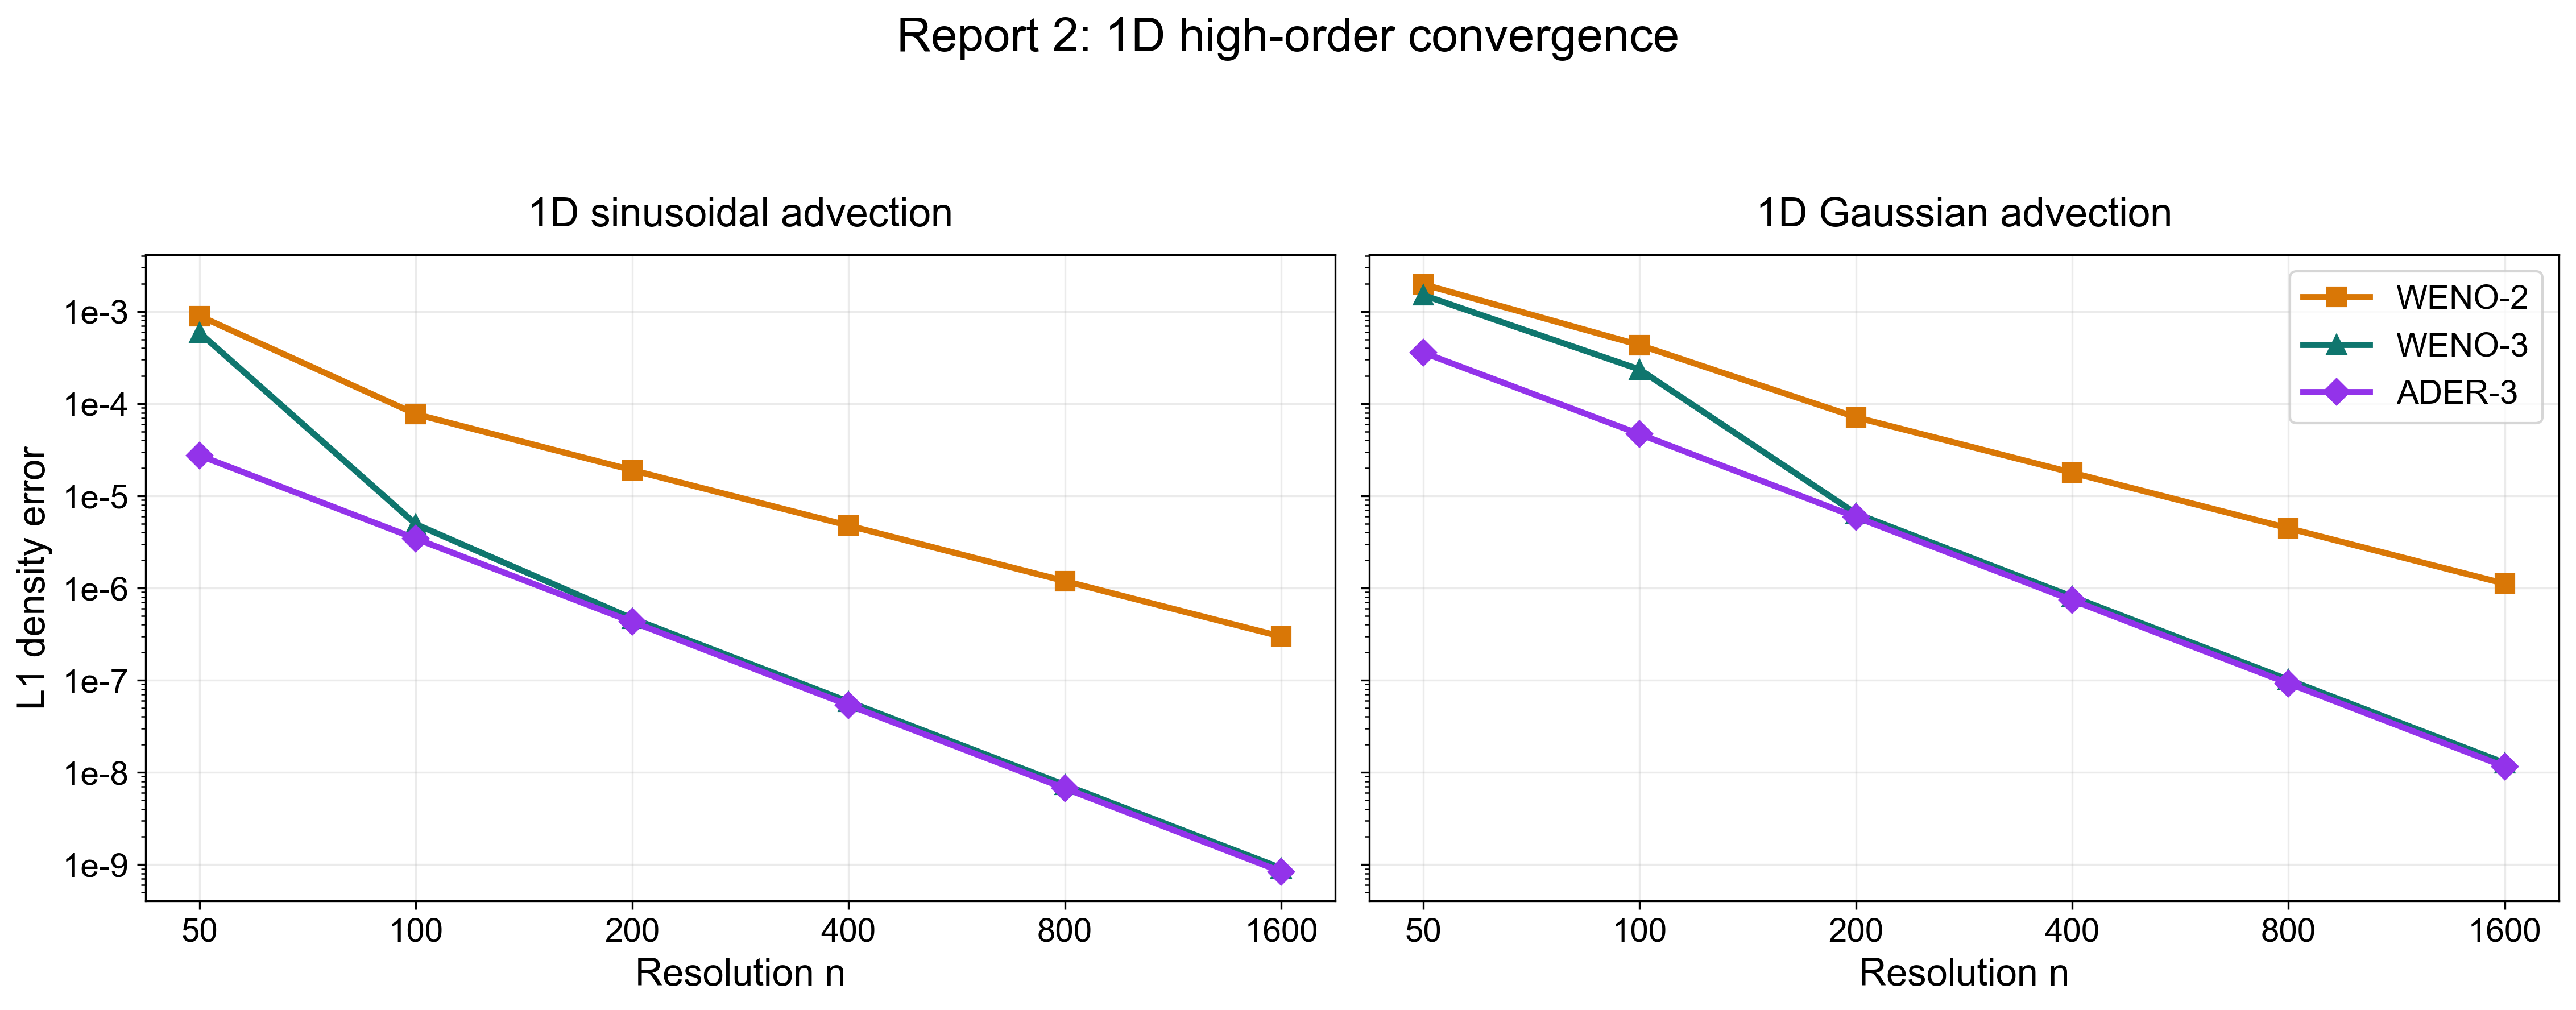
\includegraphics[width=0.97\textwidth]{convergence_1d_l1.png}
\caption{One-dimensional convergence for the smooth and Gaussian advection
profiles. Both axes are logarithmic and the plotted error is \(L_1(\rho)\).}
\label{fig:conv1d}
\end{figure}

\begin{table}[H]
\centering
\small
\setlength{\tabcolsep}{4.2pt}
\renewcommand{\arraystretch}{1.13}
\begin{tabular}{@{}r rr rr rr@{}}
\toprule
& \multicolumn{2}{c}{WENO-2} & \multicolumn{2}{c}{WENO-3}
& \multicolumn{2}{c}{ADER-3} \\
\cmidrule(lr){2-3}\cmidrule(lr){4-5}\cmidrule(l){6-7}
\(n\) & \(L_1(\rho)\) & order & \(L_1(\rho)\) & order
& \(L_1(\rho)\) & order \\
\midrule
50  & \(8.9477\times10^{-4}\) & --    & \(5.8867\times10^{-4}\) & --
    & \(2.7426\times10^{-5}\) & -- \\
100 & \(7.7022\times10^{-5}\) & 3.538 & \(4.9193\times10^{-6}\) & 6.903
    & \(3.4307\times10^{-6}\) & 2.999 \\
200 & \(1.9005\times10^{-5}\) & 2.019 & \(4.6707\times10^{-7}\) & 3.397
    & \(4.2911\times10^{-7}\) & 2.999 \\
400 & \(4.7553\times10^{-6}\) & 1.999 & \(5.8396\times10^{-8}\) & 3.000
    & \(5.3643\times10^{-8}\) & 3.000 \\
800 & \(1.1888\times10^{-6}\) & 2.000 & \(7.2996\times10^{-9}\) & 3.000
    & \(6.7055\times10^{-9}\) & 3.000 \\
1600 & \(2.9720\times10^{-7}\) & 2.000 & \(9.1246\times10^{-10}\) & 3.000
     & \(8.3818\times10^{-10}\) & 3.000 \\
\bottomrule
\end{tabular}
\caption{One-dimensional smooth-advection \(L_1(\rho)\) errors. Each order is
measured relative to the preceding grid.}
\label{tab:conv1d-smooth}
\end{table}

\begin{table}[H]
\centering
\small
\setlength{\tabcolsep}{4.2pt}
\renewcommand{\arraystretch}{1.13}
\begin{tabular}{@{}r rr rr rr@{}}
\toprule
& \multicolumn{2}{c}{WENO-2} & \multicolumn{2}{c}{WENO-3}
& \multicolumn{2}{c}{ADER-3} \\
\cmidrule(lr){2-3}\cmidrule(lr){4-5}\cmidrule(l){6-7}
\(n\) & \(L_1(\rho)\) & order & \(L_1(\rho)\) & order
& \(L_1(\rho)\) & order \\
\midrule
50  & \(1.9730\times10^{-3}\) & --    & \(1.5073\times10^{-3}\) & --
    & \(3.5844\times10^{-4}\) & -- \\
100 & \(4.3245\times10^{-4}\) & 2.190 & \(2.3519\times10^{-4}\) & 2.680
    & \(4.6774\times10^{-5}\) & 2.938 \\
200 & \(7.1327\times10^{-5}\) & 2.600 & \(6.4408\times10^{-6}\) & 5.190
    & \(5.8872\times10^{-6}\) & 2.990 \\
400 & \(1.7811\times10^{-5}\) & 2.002 & \(8.0646\times10^{-7}\) & 2.998
    & \(7.3746\times10^{-7}\) & 2.997 \\
800 & \(4.4526\times10^{-6}\) & 2.000 & \(1.0086\times10^{-7}\) & 2.999
    & \(9.2222\times10^{-8}\) & 2.999 \\
1600 & \(1.1131\times10^{-6}\) & 2.000 & \(1.2609\times10^{-8}\) & 3.000
     & \(1.1529\times10^{-8}\) & 3.000 \\
\bottomrule
\end{tabular}
\caption{One-dimensional Gaussian-advection \(L_1(\rho)\) errors. Each order
is measured relative to the preceding grid.}
\label{tab:conv1d-gaussian}
\end{table}

Both profiles give the intended asymptotic behaviour. WENO-2 settles to
second order, while WENO-3 and ADER-3 settle to third order over the finest
intervals. The isolated WENO-3 orders of 6.903 in
Table~\ref{tab:conv1d-smooth} and 5.190 in
Table~\ref{tab:conv1d-gaussian} are local pre-asymptotic transitions, not
evidence of a sixth- or fifth-order method. On these grids the nonlinear WENO
weights are moving towards their optimal smooth-flow values, while leading
spatial and temporal error components can partially cancel. Since an
observed order is computed from only two consecutive errors, that change in
the leading error coefficient temporarily produces a steep slope.

More generally, local orders on the coarsest meshes need not equal the formal
order. A smooth profile is then represented by relatively few cells, the WENO
smoothness weights have not yet reached their optimal linear limits, and
spatial, temporal, phase, and amplitude errors can have comparable sizes.
Refinement suppresses the higher error terms until a single leading term
\(C h^p\) dominates, where \(h\) is the grid spacing, \(p\) is the formal
order, and \(C\) is a grid-independent leading-error coefficient.
Consequently, the order claim is based on the stable
fine-grid sequence and its normalised-error plateau, rather than on an average
that would mix pre-asymptotic and asymptotic intervals.

The subsequent data distinguish this effect from a failed convergence test.
For smooth advection, \(L_1(\rho)n^3\) is 3.737 throughout
\(n=200,400,800,1600\). For Gaussian advection it is 51.53, 51.61, 51.64,
and 51.65.
Multiplication by \(n^3\) removes the expected third-order grid dependence,
so a nearly constant value is the estimated leading coefficient rather than
another error norm. These nearly constant normalised errors demonstrate a stable \(n^{-3}\)
asymptote. The anomalous local slopes are therefore retained as part of the
measured transition, but the formal conclusion is taken from the stable fine
grid sequence rather than from a single coarse-to-fine interval.

\section{Two-dimensional confirmation}

The two-dimensional cell-averaged Gaussian benchmark provides a concise
multidimensional check at \(t=0.1\). Rather than repeating the full 1D
refinement discussion, Figure~\ref{fig:conv2d} shows the complete refinement
sequence. The 1D results show that formal order is most reliably measured once
the grid is sufficiently fine, so Table~\ref{tab:conv2d} concentrates on the
three intervals from \(200^2\) to \(1600^2\). The reference values are exact
finite-volume cell averages, and the official smooth CFL values are used.

\begin{figure}[H]
\centering
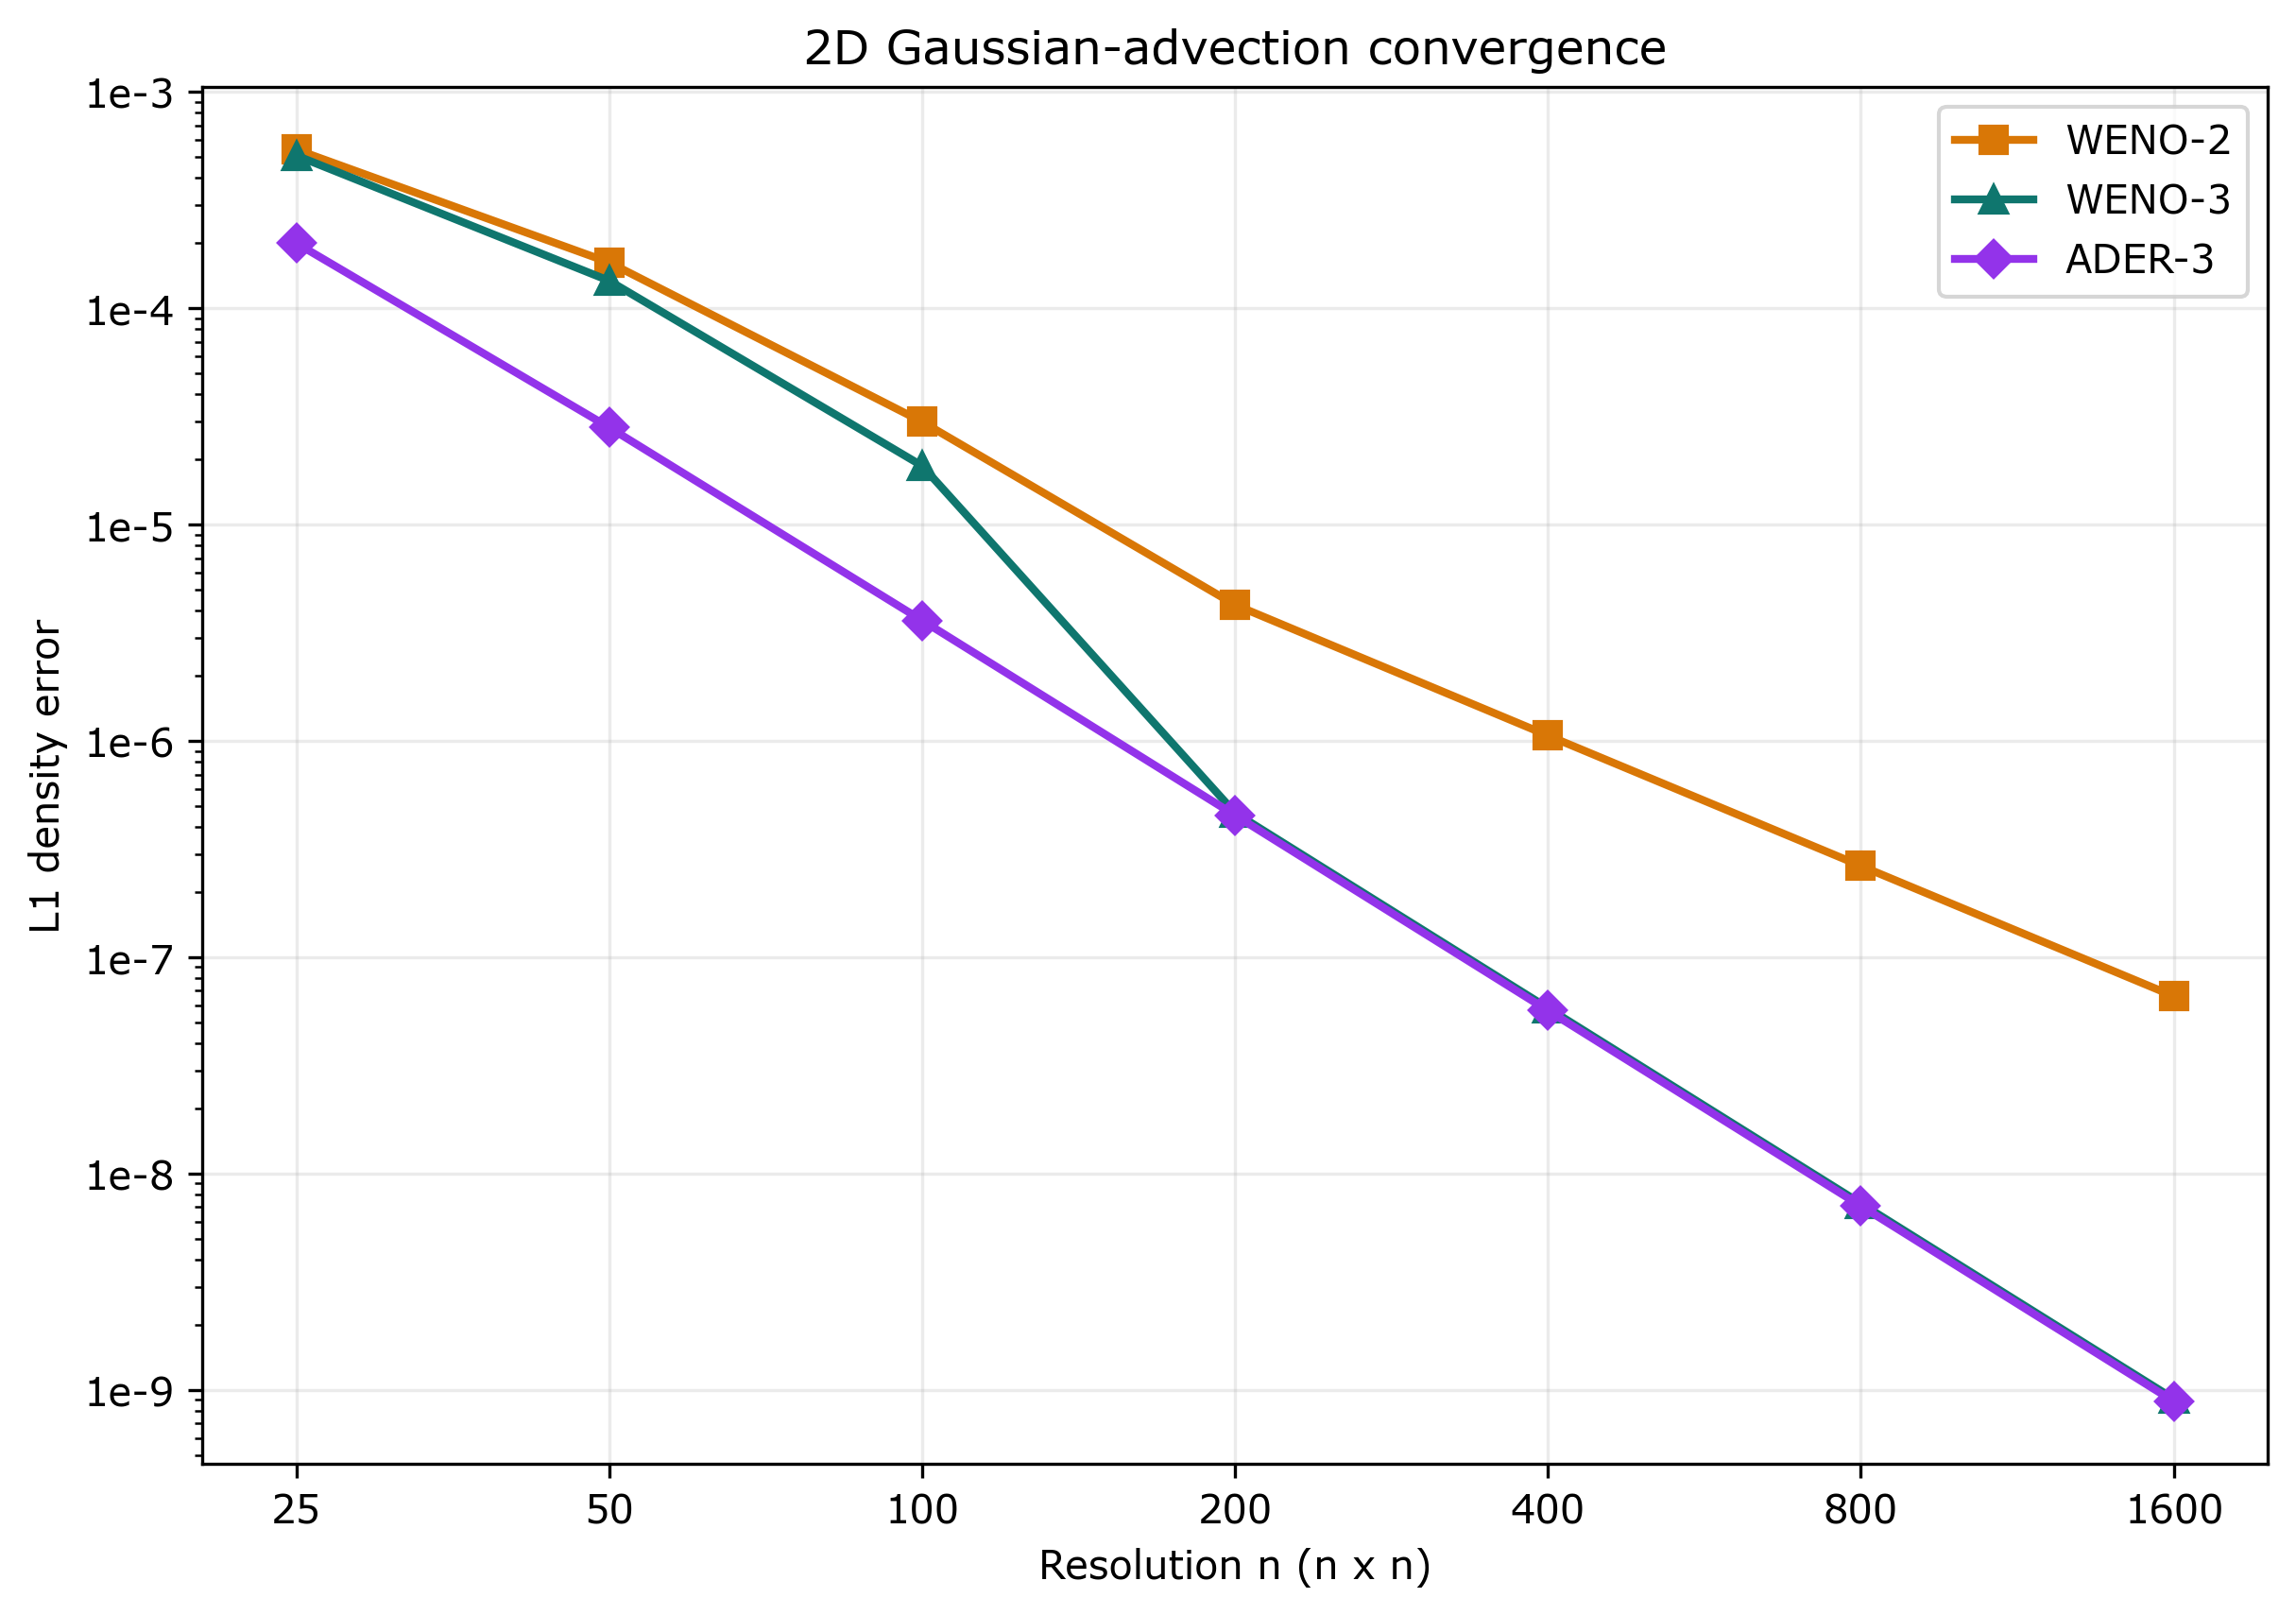
\includegraphics[width=0.86\textwidth]{convergence_2d_l1.png}
\caption{Two-dimensional Gaussian-advection \(L_1(\rho)\) convergence over
the complete \(25^2\)-to-\(1600^2\) refinement sequence.}
\label{fig:conv2d}
\end{figure}

All three errors decrease monotonically. WENO-2 settles onto its second-order
trend, while WENO-3 and ADER-3 become parallel on the fine grids and follow a
third-order trend. The unusually steep WENO-3 segment between \(100^2\) and
\(200^2\) is the same pre-asymptotic cancellation effect discussed above. It
is not interpreted as fifth-order convergence. The final three intervals
therefore provide the clean quantitative comparison.

\begin{table}[H]
\centering
\renewcommand{\arraystretch}{1.15}
\begin{tabular}{lrrrr}
\toprule
Method & \(p_{200\to400}\) & \(p_{400\to800}\) & \(p_{800\to1600}\)
& \(L_1(\rho)\) at \(1600^2\) \\
\midrule
WENO-2 & 2.007 & 2.001 & 2.000 & \(6.6102\times10^{-8}\) \\
WENO-3 & 2.998 & 3.000 & 3.000 & \(9.1051\times10^{-10}\) \\
ADER-3 & 2.998 & 3.000 & 3.000 & \(8.8664\times10^{-10}\) \\
\bottomrule
\end{tabular}
\caption{Fine-grid two-dimensional Gaussian-advection \(L_1(\rho)\) orders.
Each order is measured relative to the preceding grid.}
\label{tab:conv2d}
\end{table}

Across all three fine-grid intervals, the multidimensional result independently
recovers second order for WENO-2 and third order for WENO-3 and ADER-3. The
stability of these consecutive slopes confirms that the methods have entered
their asymptotic regimes, rather than merely producing one favourable order
estimate. On the \(1600^2\) grid, the two
third-order methods reduce the \(L_1\) density error by factors of 72.6 and
74.6 relative to WENO-2, and their errors differ by only 2.7 percent. This
fine-grid confirmation is sufficient to show that multidimensional flux
divergence and the ADER space--time construction preserve the orders already
established by the more complete 1D studies.
